% This is "sig-alternate.tex" V2.1 April 2013
% This file should be compiled with V2.5 of "sig-alternate.cls" May 2012
%
% This example file demonstrates the use of the 'sig-alternate.cls'
% V2.5 LaTeX2e document class file. It is for those submitting
% articles to ACM Conference Proceedings WHO DO NOT WISH TO
% STRICTLY ADHERE TO THE SIGS (PUBS-BOARD-ENDORSED) STYLE.
% The 'sig-alternate.cls' file will produce a similar-looking,
% albeit, 'tighter' paper resulting in, invariably, fewer pages.
%
% ----------------------------------------------------------------------------------------------------------------
% This .tex file (and associated .cls V2.5) produces:
%       1) The Permission Statement
%       2) The Conference (location) Info information
%       3) The Copyright Line with ACM data
%       4) NO page numbers
%
% as against the acm_proc_article-sp.cls file which
% DOES NOT produce 1) thru' 3) above.
%
% Using 'sig-alternate.cls' you have control, however, from within
% the source .tex file, over both the CopyrightYear
% (defaulted to 200X) and the ACM Copyright Data
% (defaulted to X-XXXXX-XX-X/XX/XX).
% e.g.
% \CopyrightYear{2007} will cause 2007 to appear in the copyright line.
% \crdata{0-12345-67-8/90/12} will cause 0-12345-67-8/90/12 to appear in the copyright line.
%
% ---------------------------------------------------------------------------------------------------------------
% This .tex source is an example which *does* use
% the .bib file (from which the .bbl file % is produced).
% REMEMBER HOWEVER: After having produced the .bbl file,
% and prior to final submission, you *NEED* to 'insert'
% your .bbl file into your source .tex file so as to provide
% ONE 'self-contained' source file.
%
% ================= IF YOU HAVE QUESTIONS =======================
% Questions regarding the SIGS styles, SIGS policies and
% procedures, Conferences etc. should be sent to
% Adrienne Griscti (griscti@acm.org)
%
% Technical questions _only_ to
% Gerald Murray (murray@hq.acm.org)
% ===============================================================
%
% For tracking purposes - this is V2.0 - May 2012

\documentclass{sig-alternate-05-2015}

\makeatletter
\def\@copyrightspace{\relax}
\makeatother

\begin{document}
\renewcommand{\qed}{}
% Copyright
%\setcopyright{acmcopyright}
%\setcopyright{acmlicensed}
%\setcopyright{rightsretained}
%\setcopyright{usgov}
%\setcopyright{usgovmixed}
%\setcopyright{cagov}
%\setcopyright{cagovmixed}
\setcopyright{none}
\pagestyle{plain} % removes running headers



%
% --- Author Metadata here ---
%\conferenceinfo{Holmblad}{'18 Winona, Minnesota USA}
%\CopyrightYear{2018} % Allows default copyright year (20XX) to be over-ridden - IF NEED BE.
%\crdata{0-12345-67-8/90/01}  % Allows default copyright data (0-89791-88-6/97/05) to be over-ridden - IF NEED BE.
% --- End of Author Metadata ---

\title{Chaotic Random Number Generation.}
%
% You need the command \numberofauthors to handle the 'placement
% and alignment' of the authors beneath the title.
%
% For aesthetic reasons, we recommend 'three authors at a time'
% i.e. three 'name/affiliation blocks' be placed beneath the title.
%
% NOTE: You are NOT restricted in how many 'rows' of
% "name/affiliations" may appear. We just ask that you restrict
% the number of 'columns' to three.
%
% Because of the available 'opening page real-estate'
% we ask you to refrain from putting more than six authors
% (two rows with three columns) beneath the article title.
% More than six makes the first-page appear very cluttered indeed.
%
% Use the \alignauthor commands to handle the names
% and affiliations for an 'aesthetic maximum' of six authors.
% Add names, affiliations, addresses for
% the seventh etc. author(s) as the argument for the
% \additionalauthors command.
% These 'additional authors' will be output/set for you
% without further effort on your part as the last section in
% the body of your article BEFORE References or any Appendices.

%\numberofauthors{8} %  in this sample file, there are a *total*
% of EIGHT authors. SIX appear on the 'first-page' (for formatting
% reasons) and the remaining two appear in the \additionalauthors section.
%
\author{
% You can go ahead and credit any number of authors here,
% e.g. one 'row of three' or two rows (consisting of one row of three
% and a second row of one, two or three).
%
% The command \alignauthor (no curly braces needed) should
% precede each author name, affiliation/snail-mail address and
% e-mail address. Additionally, tag each line of
% affiliation/address with \affaddr, and tag the
% e-mail address with \email.
%
% 1st. author
\alignauthor
Michael Holmblad \\
       \affaddr{Winona State University}\\
       \affaddr{175 W Mark St, Winona MN 55987}\\
       \affaddr{Winona State University}\\
       \email{mholmblad13@winona.edu}
}
% There's nothing stopping you putting the seventh, eighth, etc.
% author on the opening page (as the 'third row') but we ask,
% for aesthetic reasons that you place these 'additional authors'
% in the \additional authors block, viz.
\date{27 April 2018}
% Just remember to make sure that the TOTAL number of authors
% is the number that will appear on the first page PLUS the
% number that will appear in the \additionalauthors section.

\maketitle
\begin{abstract}
	This paper focuses on creating and testing a pseudo random number generator (pRNG) using a branch of mathematics known as chaos theory. Generators are created based off of several chaotic systems. This paper goes through the process of how the tent map was chosen and modified to create a good rng. There has been research on the tent map as a generator, but not in this kind of sense. The tent map has had natural problems with computer hardware in the past, but those deficiencies were taken care of. This paper analyzes that creation process and tries to categorize the generator that was created.
	
\end{abstract}


%
% The code below should be generated by the tool at
% http://dl.acm.org/ccs.cfm
% Please copy and paste the code instead of the example below. 
%
%\begin{CCSXML}
%<ccs2012>
 %<concept>
  %<concept_id>10010520.10010553.10010562</concept_id>
  %<concept_desc>Computer systems organization~Embedded systems</concept_desc>
  %<concept_significance>500</concept_significance>
 %</concept>
 %<concept>
  %<concept_id>10010520.10010575.10010755</concept_id>
  %<concept_desc>Computer systems organization~Redundancy</concept_desc>
  %<concept_significance>300</concept_significance>
 %</concept>
 %<concept>
  %<concept_id>10010520.10010553.10010554</concept_id>
  %<concept_desc>Computer systems organization~Robotics</concept_desc>
  %<concept_significance>100</concept_significance>
 %</concept>
 %<concept>
  %<concept_id>10003033.10003083.10003095</concept_id>
  %<concept_desc>Networks~Network reliability</concept_desc>
  %<concept_significance>100</concept_significance>
 %</concept>
%</ccs2012>  
%\end{CCSXML}

%\ccsdesc[500]{Computer systems organization~Embedded systems}
%\ccsdesc[300]{Computer systems organization~Redundancy}
%\ccsdesc{Computer systems organization~Robotics}
%\ccsdesc[100]{Networks~Network reliability}


%
% End generated code
%

%
%  Use this command to print the description
%
%\printccsdesc

% We no longer use \terms command
%\terms{Theory}

%\keywords{ACM proceedings; \LaTeX; text tagging}

\section{Introduction}
\noindent
Random number generation (RNG) has been around for a very long time. Ever since a person spoke the words "heads or tails", people have been randomly generating numbers. One of the most used random number generators on the planet is a die or the usage of multiple dice. Items such as coins, dice, and similar random chance methods are known as true random number generators. (tRNG) These generators are used to pull a truly random number, and if made correctly, perform that task perfectly. However, humans have been trying to replicate this process on a computer ever since they started making video games, protecting information, and any other task that involves the usage of a random number. These generators are often known as pseudo random number generators. (pRNG) It must be asked, what is are random numbers?
\newdef{definition}{Definition}
\begin{definition}
	\textit{Random numbers} are numbers that occur in a sequence such that two conditions are met: (1) the values are uniformly distributed over a defined interval or set, and (2) it is impossible to predict future values based on past or present ones.
\end{definition}
The goal of this paper is to educate about random number generators and to create a computerized tRNG, or at least come as close as possible to creating one.

\section{Background Research}
\noindent
\subsection{Theory}
\noindent
Pseudo random number generation has been a discussion topic in mathematical computer science for a very long time. One book that people often refer to for information on pseudo random number generation is "The Art of Computer Programming" which is written by Donald Knuth. [3] He describes the creation of one of the most popular original pRNGs known as the Linear Congruential method, which is discussed a little later from now. 

\noindent
One thing about pRNGs that is talked about are their period length. 
\begin{definition}
	A \textit{period} is the length of the string generated before it repeats a generated number.
\end{definition}
The longer a period, the better the generator. Long is arbitrary though in this case, as in, there must be a long enough period to satisfy the needs of the generator's purpose. 

\noindent
Another topic that Donal Knuth talks about is seeds. 
\begin{definition}
	A \textit{seed} is a number or vector used to initialize a pseudo random number generator.
\end{definition}
Seeds can have an impact on how well pRNGs work. Every seed gives its own form of output. To abuse a pRNG correctly, we must choose a seed that generates the longest period, and similar seeds like it. However, in the realm of chaos theory, this isn't a problem. No seed should have a distinct advantage over another. Thus, generators must have seed choice irrelevance.
\subsubsection{Linear Congruential Method}
\noindent
This is the most flushed out RNG in the research of RNGs. It has a very simple formula, $$X_{n+1} = (aX_n + c) \mod m.$$
What should be noted is that $X$ is the sequence, $a$ is some multiplier, $c$ is an increment, and $m$ is a modulus to keep the numbers in a certain range. This method showed the importance of long periods and picking the correct seed. It proved that choosing a good seed can make or break the generator. It was also decided that seed choice must be avoided at this point.

\section{Chaos Theory and its Role}
\noindent
Chaos theory plays a very important role in the discovery of this new method to generate pseudo random numbers. A Chaotic Dynamical System has two major properties. According to Robert Devaney, 
\begin{definition}
	A dynamical system is \textit{chaotic} if it satisfies three conditions: transitivity, have a dense set of periodic points, and sensitive dependence on initial conditions. 
\end{definition}
This definition is the widely accepted definition on what it means to be chaotic. The funny thing, is that this definition also defines a random number generator in some odd way. These three conditions can be compressed into two well defined requirements.

\noindent
The first of these two requirements is \textit{sensitive dependence on initial conditions}; each point in a chaotic system is arbitrarily closely approximated by other points with significantly different future paths, or trajectories. Thus, an arbitrarily small change, or perturbation, of the current trajectory may lead to significantly different future behavior. A more simple definition is that arbitrarily close seeds create widely diverging sequences. This is key to generating random numbers because as long as the seeds are not exactly equal, they should be extremely different. Thus establishing a requirement denoted as \textit{practical unpredictability}, given any sequence without the equation for the generator, it should be nearly impossible to predict the next term no matter how long the sequence is. Thus, if the system is chaotic, then it has sensitivity to initial conditions, and therefore has practical unpredictability.

\noindent
The second of these two major requirements is that a chaotic system must have a \textit{dense orbit}; every point in the space is approached arbitrarily closely by periodic orbits. A \textit{periodic orbit} is a point which the system returns to after a certain number of function iterations or a certain amount of time. The dense orbit contains many different periodic orbits, thus creating long periods, seed choice irrelevance, and possibly a uniform distribution.

\section{Methodology}
\noindent
This project is designed to take the chaotic system known as the tent map and turn it into a generator. The steps are to modify it so that the computer can preserve the chaotic properties of this mapping. Then once the generator is coded, it must be tested. There are many testing suites out there to test random number generators, however the most recognized testing suite is the dieharder test suite. The dieharder test suite is made up of three other test suites, plus more tests made by the creator of the suite. 
\subsection{Coding}
\noindent
There was a major challenge that came with producing all of the code for this project. This project utilized two different languages throughout the process. For all the preliminary setup work, python was chosen for its ability to create histograms in as little code as possible. For the generator creation and testing, C was chosen because of how close it relates to the hardware.
\subsubsection{Python Theoretical Portion}
\noindent
During the python portion there were a couple things that needed to be done and led to python being chosen for these tasks. Python has a plethora of packages for doing simple mathematical calculations with the numpy library. On the other side of that coin, there is the robust plotting library known as seaborn, which was used to make all of the histograms in this paper. 

\noindent
The first system that was analyzed is known as the Logistic map. To be even more specfic, it was the logistic map of degree $4$, $4x(1-x)$. It is one of the most recognized chaotic systems. After plotting a distribution for it on the interval $[0,1]$, the logistic map was abandoned as the ulam distribution pictured below appeared.
\begin{center}
	\begin{figure}[h]
		\center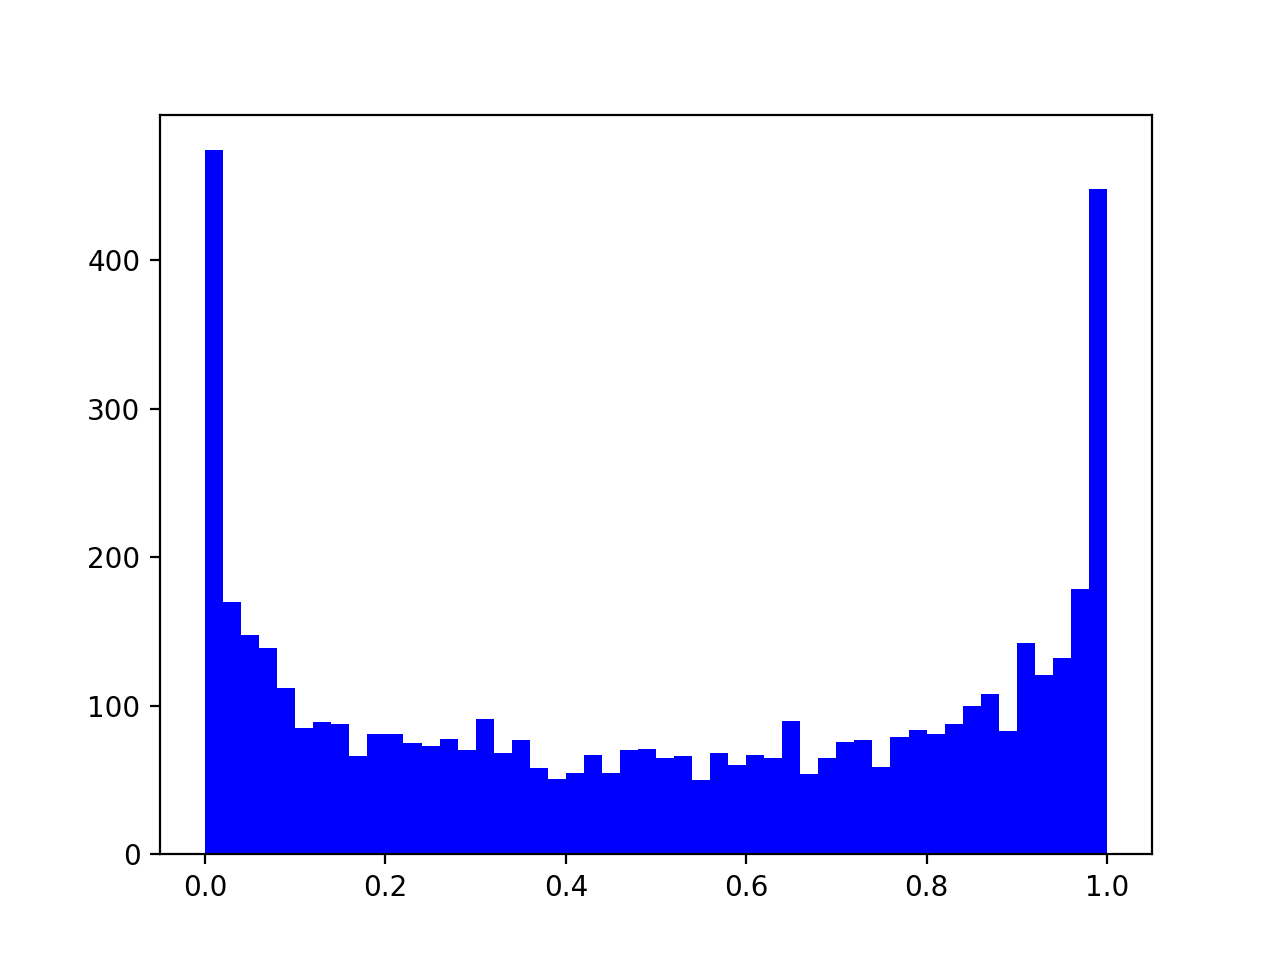
\includegraphics[width=3in]{Ulam}
		\caption{Ulam distribution for the logistic map}
	\end{figure}	
\end{center}
Seeing as that distribution isn't uniform, it was decided that the system must be more linear. Thus, the tent map was chosen as the next system to examine.

\noindent
The tent map is as follows,
$$f(x)=\begin{cases}
2x & 0 \leq x\leq \frac{1}{2} \\
2-2x & \frac{1}{2} < x\leq 1
\end{cases}.$$
Then a histogram was plotted to check to see if this distribution was uniform as well.
\begin{center}
	\begin{figure}[h]
		\center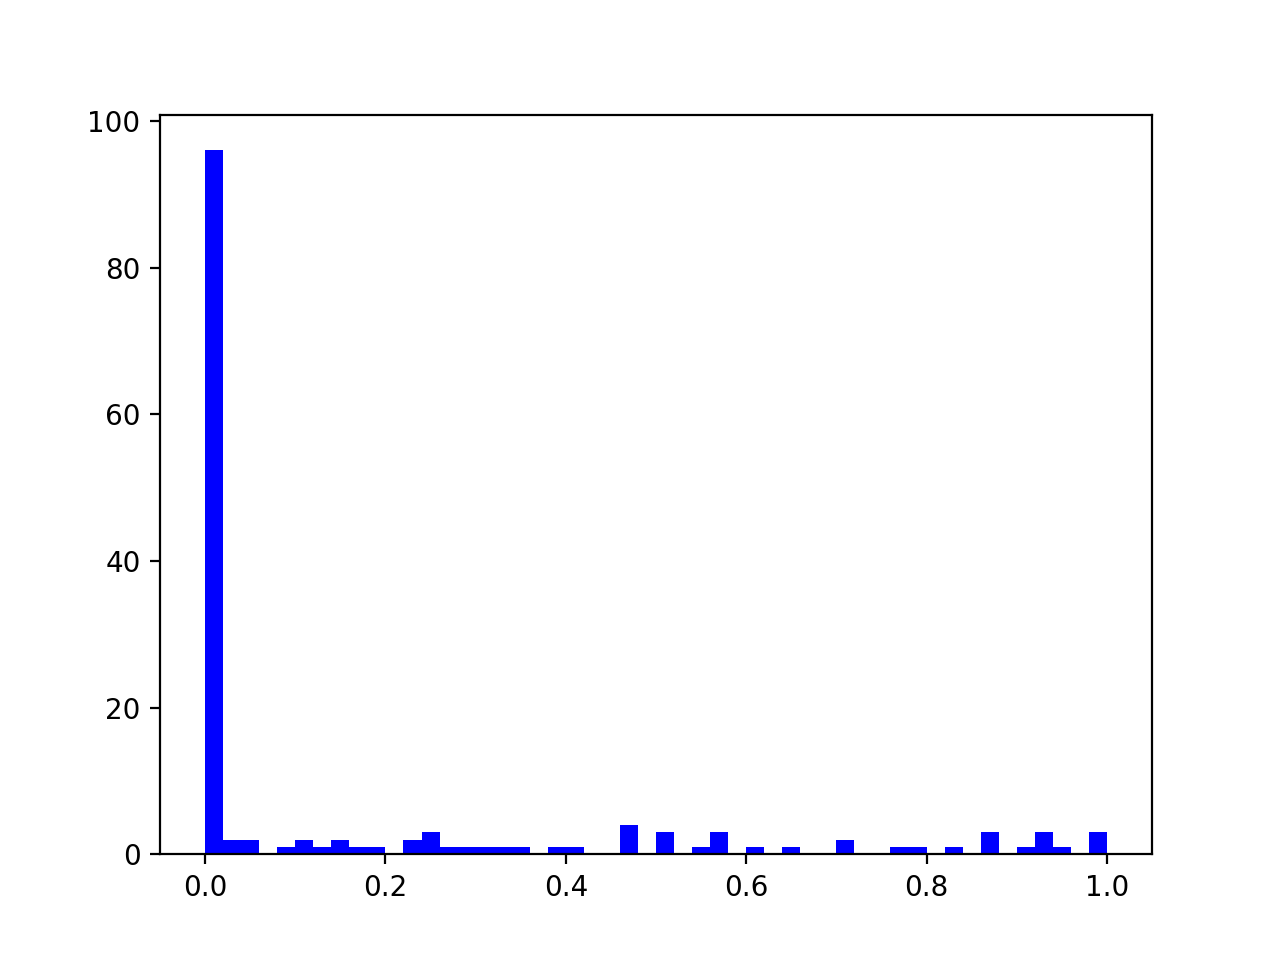
\includegraphics[width=3in]{tent150}
		\caption{Distribution for the tent map after plotting 150 iterates}
	\end{figure}
\end{center}
Seeing as this distribution had a ton of zeros, and a very balanced amount spread throughout the rest of the chart, something seemed off. It was then discovered that IEEE released a floating point standard in 1985. This standard says that floating point words are made up of 52 fraction bits, 11 exponent bits, and 1 sign bit. It just so happens that the tent map is equivalent to a bit shift map on the interval $[0, \frac{1}{2}]$. The map is also simultaneously a bit shift and bit flip map on the interval $[\frac{1}{2}, 1]$, since the map is base two, it will zero out guaranteed at the $54^{th}$ iterate. The standard did not change how $64-bit$ words were organized since then. Note, that the tent map will zero out once the number fraction bits is exceeded. Thus, this is a hardware problem. This became dubbed as the bit-loss problem. Proofs are in the appendix to show the mathematics behind this problem.

\noindent
The trick became solving the bit-loss problem while also preserving the properties of the tent map. The answer was simple, instead of two sections, break the tent map into three sections.
$$f(x)=\begin{cases}
3x & 0 \leq x\leq \frac{1}{3} \\
2-3x & \frac{1}{3} < x\leq \frac{2}{3} \\
3x-2 & \frac{2}{3} < x \leq 1
\end{cases}.$$
A proof was then written to show two things, the tent $3$ map is chaotic, and the tent $3$ map is a ternary shift. Once these proofs were written, it the tent $3$ map had to be plotted on a computer to verify the proofs.

\begin{center}
	\begin{figure}[h]
		\center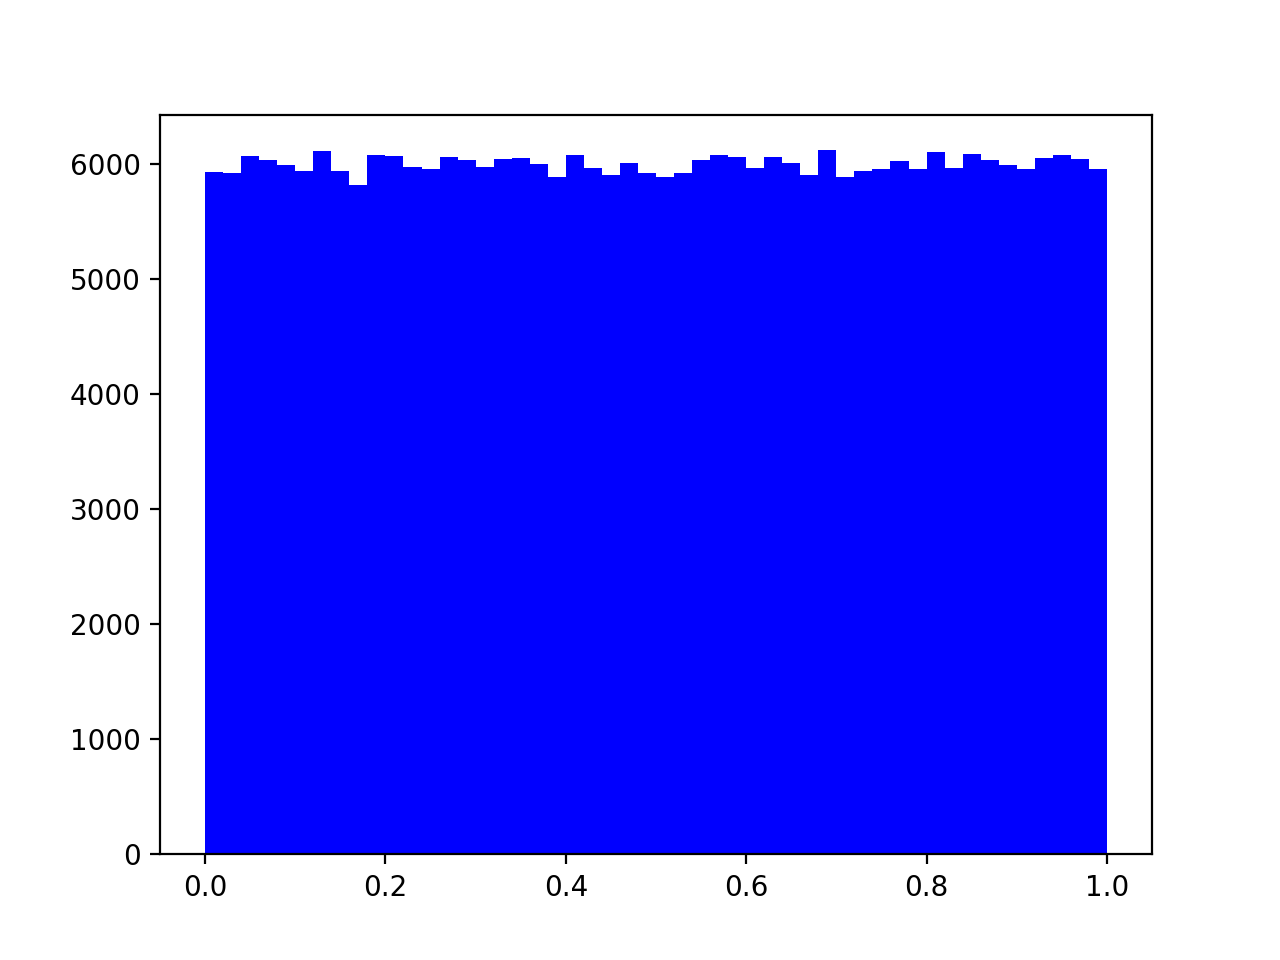
\includegraphics[width=3in]{tent300000}
		\caption{Tent 3 map after 300000 iterates}
	\end{figure}
\end{center}
\noindent
As can be seen by the above distribution, the system is uniform. To put everything together, since the tent map is chaotic and creates a uniform distribution all requirements are theoretically met. The map has sensitivity to initial conditions, dense orbits, and it is linear. Thus, it has practical unpredictability, seed choice irrelevance, seemingly infinite periods, and a uniform distribution. But, of course, it must be put to the test.

\subsection{C Application Portion}
\noindent
The chaotic tent 3 map doesn't get destroyed by a computer like the original tent map. The tent 3 map hasn't been programmed as a generator before, so that must be figured out next. Thankfully, there is the general scientific library (gnu scientific library) that was written in C. This library supplies many different methods for the initialization, seed generation, tear down, and output capabilities for making a good generator. 

\noindent
The next thing that had to be solved is how does it get tested?  The best way to test a generator is to pick a good statistical test suite. Dieharder is a statistical test suite that was created by Robert G. Brown, who is a professor at Duke University. [1] This test suite is comprised of several different test suites, which are the original diehard tests, the NIST test suite, the statistical test suite (sts), and tests made by Dr. Brown himself. Of course, the usefullness of all these different tests overlap with one another, but it is extremely useful to have all $114$ different tests. To add to the thoroughness, dieharder will the tests multiple times to generate a large pool of results. The one complication here is the data type. The dieharder test suite requires a text file or a binary file full of numbers from $0$ to $MAX\_INT$. Of course, it wants $UINT\_MAX$, and the integers have to be $32$-bit integers The complication then becomes a matter of converting from an integer(seed) to a float(calculations) and then back to an integer(output) again. This matter became trivial after thinking about how the architecture works. If we want to have a file full of $32$-bit signed integers and the float data types are $32$-bit, then seven bits of exponent are lost when switching from float back to int. The fix is to do all the calculations in $64$-bit words, bits will still be "lost" converting from int to float to int, but they will be lost anyway going from $64$-bit to $32$-bit words. The key was to trick the computer into only returning the signed $32$-bit portion of the $64$-bit, then the output would be all $32$-bit integers that are on the range $[0, Max\_Int]$

\noindent
Needless to say, that silly fix solved all the precision problems. Just like changing the mod to solve the zero out problem, moving up an order of bit magnitude solved the storage and type conversion problem. Thus, the generator was finally able to be tested.

\section{Results and Analysis}
\noindent
Needless to say, all the dieharder tests were passed by both the mod 3 map, and by the mod 3 tent map. The results are comparable to the Mersenne Twister known as mt19937, and the $AES\_OFB$ generator. The dieharder tests outputs a bunch of p-values for each statistical test. Then they are categorized into three broad categories of passed, weak, and failed. Passed gives a value, failed returns zero, and weak returns a ridiculously high or a ridiculously low p-value


\begin{center}
	\begin{table}[h]
		\caption{Some Dieharder output}
		\center\includegraphics[width=3.5in]{output}
	\end{table}
\end{center}
\noindent
The important thing to look at with the table on the next page, are the p-values. Not specifically analyzing how they directly compare, because they are going to come out different every time. The reason for that is the numbers are sampled from the generator and then sampled by the test, and those elements are going to change every time. The important thing to note is that a weak result every so often, and a failed every so often are a good thing. The problem is when they happen all the time. The different generators that were tested return a wide range of values, but they are widespread enough to where it isn't a serious problem. In fact, these results are assumed to be correct behavior. The results show an assortment of the average p-values wanted which is in the range of $.4$ to $.6$, outliers around $.05$ and $.95$ which are wanted a very small amount of the time, but still wanted and then every other kind of value in between.

\noindent
Thus, one could argue at the moment, that this chaotic system full of mathematical bit shifts and taking the complement, is comparable to AES and the most respected Mersenne Twister. However, these generators are more well respected because of how long they have been used in industry. The AES generator and the Mersenne twister generator have been around for 10 - 20 years each. This has given them plenty of time to be repeatedly tested and repeatedly used, thus building its reputation.


\section{Conclusion}
\noindent
Throughout this project there have been several discoveries that cannot go unnoticed. The first one is how data type conversions are more precise when 32 bit words are getting stored into 64 bit words when converting between floats and integers. The next major key here is how a theoretically perfect map can "zero out" on a computer due to its nature, but somehow be modified to achieve the overall goal. The last lesson is that theoretically perfect only works if there is a simple way to preserve the purity of the system in practice. Otherwise, theoretically perfect will never equal possible, until a practical method is discovered. It is still amazing that such a simple function design works this well as a generator at the time this paper is written. The final result is that for now, this generator is successful, but it must be continually tested and keep doing well.


%ACKNOWLEDGMENTS are optional
\section{Acknowledgments}
\noindent
Special thank you to the main advisor of this project Dr. Peratt who guided this research process through to the end. Special thank you to Dr. Iyengar and Dr. Zhang, who guided and helped question the methodology and practices in this research. Special thank you to all Winona State faculty and colleagues that would listen to babbling about this project.

\begin{thebibliography}{1}
	\bibitem{1st} Brown, Robert G. {\em dieharder} Duke University Physics Department, 19 June 2017. Web. \\
	
	\bibitem{2nd} Devaney, Robert L. {\em A first course in chaotic dynamical systems: theory and experiment} Addison-Wesley, 1999. Print. \\
	
	\bibitem{3rd} Knuth, Donald {\em The Art of Computer Programming Volume 2: Seminumerical Algorithms} Addison-Wesley, 1968. Print.  \\
	
	\bibitem{4th} Phatak, S. C., and S. Suresh Rao. {\em Logistic Map: A Possible Random-Number Generator} Physical Review E, vol. 51, no. 4, 1995. Journal.  \\
	
	\bibitem{5th} Haahr, Mads {\em RANDOM.org} RANDOM.org, October 1998. Web.

	
\end{thebibliography}

\appendix
\newdef{proposition}{Proposition}
\begin{proposition}
	The mod 2 map is a shift.
	\begin{proof}
		Suppose we have a mapping function $f(x)$, where $$f(x)=
		\begin{cases}
		2x & 0 \leq x\leq \frac{1}{2} \\
		2x-1 & \frac{1}{2} < x\leq 1
		\end{cases}$$ where $0 \leq x \leq 1$ implies that x is always some decimal number. Therefore, since computers do there calculations in binary we may represent $x$ in the form $\frac{d_1}{b^1} + \frac{d_2}{b^2} + \frac{d_3}{b^3} + ...$. So, all x values are of the form $\frac{d_1}{2^1} + \frac{d_2}{2^2} + \frac{d_3}{2^3} + ...$. 
		
		
		Now suppose that $x \leq \frac{1}{2}$, then by $f(x)$ we must multiply $x$ by $2$, which looks like, $2 \cdot (\frac{d_1}{2^1} + \frac{d_2}{2^2} + \frac{d_3}{2^3} + ...) = d_1 + \frac{d_2}{2^1} + \frac{d_3}{2^2} + \frac{d_4}{2^3} + ...$. This may be called a left shift, since all of the components of $x$ simply lost a power of $2$ in the denominator. and therefore they all have a greater value. 
		
		
		Next, suppose that $\frac{1}{2} < x \leq 1$, then by $f(x)$ we must multiply $x$ by $2$, which looks like, $2 \cdot (\frac{d_1}{2^1} + \frac{d_2}{2^2} + \frac{d_3}{2^3} + ...) = d_1 + \frac{d_2}{2^1} + \frac{d_3}{2^2} + \frac{d_4}{2^3} + ...$. But, this time we subtract $1$ as well, because $d_1 + \frac{d_2}{2^1} + \frac{d_3}{2^2} + \frac{d_4}{2^3} + ... > 1$.  Which obtains, $\frac{d_2}{2^1} + \frac{d_3}{2^2} + \frac{d_4}{2^3} + ... $. This may be called a left shift, since all of the components of $x$ simply lost a power of $2$ in the denominator. and therefore they all have a greater value. However, we also cut off the leading term so that we stay inside the range of the map, but it is still a left shift.
		
		
		Thus, the mod 2 map is a shift map. 
	\end{proof}
\end{proposition}

\newdef{corollary}{Corollary}
\begin{corollary}
	The mod 2 map and the tent map will always zero out after 54 iterations.
	\begin{proof}
		In 1985, the Institute of Electrical Electronic Engineers published IEEE $754$ (Standard of Floating Point Arithmetic) in $1985$. Thus, on all modern computers every 64-bit floating point number is divided up into $53$ coefficient bits, $11$ exponent bits, and $1$ sign bit. 
		
		
		By Proposition 1, we know that the mod 2 map and the tent map knick a term off the front, then recalculates. Since, its in binary, that bit. After 54 iterations of this we only return 0, since the floating point coefficient bits have overflowed with zeros.
		
		
		Thus, the mod 2 map and the tent map zero out on computers.
	\end{proof}
\end{corollary}

\end{document}
